\chapter{Memory Analysis}
To get a better insight on how Hive uses memory, I needed to build a basic model when and why Hive's reserved memory grows. During my work, I mainly focused on HiveServer2. The first step toward the model building was to get basic knowledge about Hive's code base and the query compilation process. The query life cycle mentioned in the previous chapter helped, but I had to find those steps in the code. If I have these points I am able to start measuring and maybe find some memory wastes.

\section{Finding the measuring points}
Hive has around 2 million lines of code so locating the main steps of the query processing was challenging. 

As a starting point, the user enters a query in the client. At this point, I run Hive locally, so the simplest way for submitting queries against Hive was using Beeline command line client. HS2 gets the query through its Thrift interface. After this, the query goes to the \textit{Driver} class, which is the main class for executing queries.

The Driver has two methods that are important for me: run and runInternal. The run method gets called first, which basically just delegates to the runInternal method. These two functions return with a CommandProcessorResponse, once the compilation and execution are done. 

\noindent The runInternal does the two main steps:
\begin{itemize}
	\item Driver.compile: gets the command string and parses, analyses the query and generates the execution plan.
	\item Driver.execute: gets the execution plan and executes it on a specific engine (MapReduce, Spark or TEZ).
\end{itemize}

\subsection{Compile}
The first step of the compilation is the parsing. It takes a string and returns an Abstract Syntax Tree (AST or the Parse Tree).

\begin{lstlisting}
public int compile(String command, ...) {
...
	ASTNode tree;
	try {
		tree = ParseUtils.parse(command, ctx);
	} catch (ParseException e) {
...
}
\end{lstlisting}
\subsubsection{Semantic Analyzis}
After the AST is generated, the compile process will continue with the semantic analyzer. The type of the analyzer will depend on the query type we are running. For SELECT and INSERT the SemanticAnalyzer class is used. 

\begin{lstlisting}
public int compile(String command, ...) {
...
	BaseSemanticAnalyzer sem = SemanticAnalyzerFactory.get(queryState, tree);
...
	sem.analyze(tree, ctx);
...
}
\end{lstlisting}

The SemanticAnalyzer class is the main phase during compilation. It checks for semantic errors, fetches metadata from Metastore, generates and optimizes the query plan. The analyze method of the BaseSemanticAnalyzer is called from the Driver's compile method, and it delegates the call to the corresponding Analyzer. From now on, I will write about the SemanticAnalyzer class and its phases (which is executed for SELECTS and INSERTS.

\begin{lstlisting}
void analyzeInternal(ASTNode ast, PlannerContext plannerCtx) {
	//(1)
	if (!genResolvedParseTree(ast, plannerCtx)) {
		return;
	}
	//(2)
	Operator sinkOp = genOPTree(ast, plannerCtx);
	...
	//(3)
	...
	resultSchema = convertRowSchemaToViewSchema(...);
	...
	//(4)
	Optimizer optm = new Optimizer();
	... = optm.optimize();
	...
	//(5)
	TaskCompiler compiler = TaskCompilerFactory.getCompiler(conf, pCtx);
	compiler.compile(pCtx, rootTasks, inputs, outputs);
	...
}
\end{lstlisting}

\begin{enumerate}
	\item Fetches metadata and fill the Parse Tree with it so it becomes a Resolved Parse Tree.
	\item The Operation Tree gets created which will contain operators that process data read from the table. This tree is called by the Map and Reduce methods.
	\item The semantic analyzer will deduce the schema of the result set from the row schema
	\item A logical optimization is done on the Operator Tree. There are two types of optimization: one that transforms the Operator Tree (like removing unnecessary operations) and one that does not (predicate pushdown, vectorization \etc).
	\item Physical optimization and translation to the target execution engine take place. The output of this stage is the query plan. It can optimize the tree according to the engine used. For example in MR, common join can be translated to map-side join, if one of the tables is small enough to fit into the memory of the map nodes.
\end{enumerate}

\begin{lstlisting}
public int compile(String command, ...) {
	...
	sem.validate();
	...
}
\end{lstlisting}

After the semantic analysis is completed, the Driver will validate the plan. When it completes, the compilation ends and Hive will continue with the execution.

\clearpage
\section{Measure the memory of HiveServer2}
If I want to measure the memory usage of Hive, I need a something to create and analyze heap dumps and generate memory statistics. There are several tools to choose from. In this section, I will present the tools I considered and the method I used to get a better understanding of HS2 memory patterns.

\subsection{Tools for generating heap dumps and statistics}
For creating heap dumps and statistics of the memory, I decided to use a command line tool. In contrast of a UI tool, it has the benefits to generate heap dumps and statistics automatically. 

\subsubsection{jmap}
\textit{jmap} \cite{jmap} can be used to obtain heap dumps and histograms from a running java process.

To gather information about a running Java program we need its process ID (PID). Using this we can easily create the heap dump with the \textit{-dump} option. If we do not want to analyze large heap dumps, just to get the objects that reserve the most memory, we can use the \textit{-histo} option. It will print a histogram of the heap, containing each Java class, the number of objects and memory sizes per class.

\subsubsection{jcmd}
\textit{jmap} would have been a perfect choice for measuring memory. However, it is recommended to use the latest utility, which is called \textit{jcmd} \cite{jcmd}. It has enhanced diagnostics capability and its perfomance overhead is reduced. 

The usage of jcmd is similar to jmap. For creating heap dumps we can use \textit{jcmd <PID> GC.heap\_dump}. If we want to obtain class histogram we can do that with the \textit{jcmd <PID> GC.class\_histogram} command. With the \textit{jcmd <PID> GC.heap\_info} command we can gather basic information of the heap: \eg young and old memory of the process.

I decided to use jcmd in my future work to gather memory information automatically and generate heap dumps at the measuring points identified in the previous section.

\subsection{Tools for analysing heap dumps}
Creating heap dumps with a CLI tool is easier, however analysing those requires a tool with user interface. 

\subsubsection{YourKit}
\textit{YourKit} provides great analysing capabilities for heap dumps. We can use it for profiling local or remote Java applications. It has controllable overhead. Although, it is a great tool for profiling Java applications, it is a commercial software and only has 15 days of free licence.

\subsubsection{VisualVM}
\textit{VisualVM} provides a great visual interface for profiling Java applications and browsing heap dumps. It offers multiple views for analysing them. We can get the summary of the dump which contains the total bytes, classes and objects. 

With the "classes view" we can get information about the reserved memory and number of instances for each class. We can calculate the retained memory, which is the memory that would be freed if the objects would be garbage collected.

\subsubsection{JXRay}
JXRay \cite{jxray} is a memory analysis tool for Java applications. It creates a HTML report of a given heap dump. It can automatically detect common problems, like data duplication or non-optimal usse of data stuctures. 

JXRay can give us a compact report, even if the heap dump analyzed is 10's of GB. It can calculate how much memory taken by a collection internal representation and their workload, since JXRay knows about the internal representation of common java collections (HashMap, ArrayList \etc).

\begin{figure}[H]
	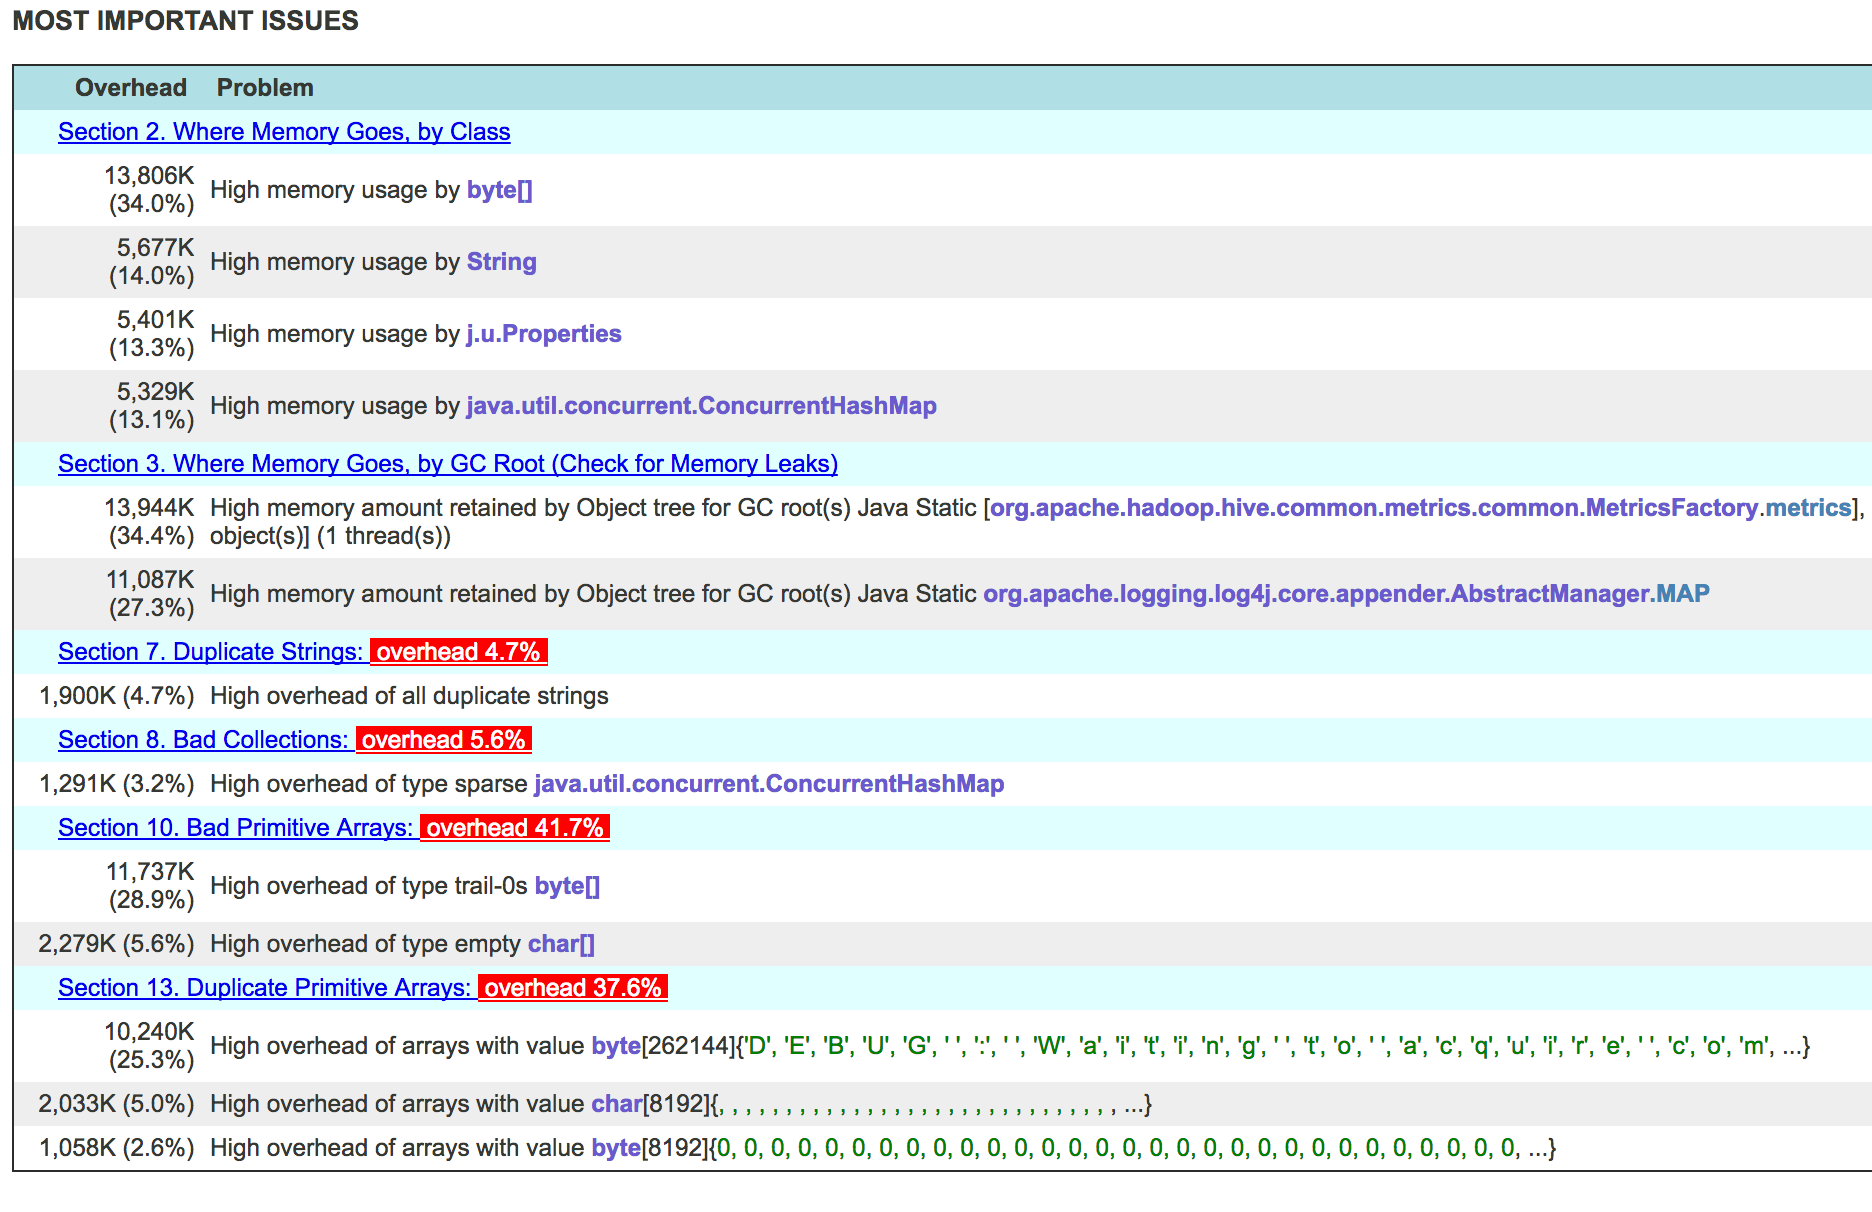
\includegraphics[width=150mm, keepaspectratio]{figures/jxray_sample.png}
	\centering
	\caption{Sample JXRay report summary}
\end{figure}

\subsubsection{The selected tool}
I decided to use VisualVM for visual memory analysis since it has great capabilities for summarizing the most important information about a heap dump and with its help, I am able to walk through the memory tree easily.

During my work, I also used JXRay, since it can automatically detect the most common memory problems and give me an overview of the possible issues a Java application has.

\clearpage
\subsection{Creating the code to measure memory}
With the available tools I am able to generate heap dumps really easily. However, to get a model how Hive uses the memory, I should gather statistics and heap dumps at certain points of the query execution. Clearly, it is not possible by hand. Thus, I needed to create a class in Hive's codebase and integrate the sampling in the identified points found in the previous section.

In order to use jcmd from Java, I needed a way to execute a terminal command from code. With the \textit{ProcessBuilder} java class I'm able to create operating system processes with the given attributes. The \textit{Runtime.exec()} method would do the same, but using this command is discouraged. 

Now that I can run a command line tool from Java, I will need the process ID of HiveServer2. Since Hive uses Java 8, I cannot use the new Process API that Java 9 provides. With the help of the \textit{ManagementFactory} class, we can get the managed bean of the runtime system of the JVM. It will return a class implementing the \textit{RuntimeMXBean} interface. The name of the running JVM contains the ID of the process. With the \textit{RuntimeMXBean.getName()} method, I was able to get the PID of HiveServer2. The method will return a string in a format of: \textit{pid@hostname}. Using the split method we can get our application's process ID.

To avoid code duplication I created a method for getting the ProcessBuilder which contains the given command and the PID for HiveServer2 is already set.

\begin{lstlisting}
private ProcessBuilder getProcessBuilder(String subCommand){
	ProcessBuilder builder = new ProcessBuilder();
	//Get own pid
	String pid = ManagementFactory.getRuntimeMXBean().getName().split("@")[0];
	builder.command("sh", "-c", String.format("jcmd %s %s", pid, subCommand));
	return builder;
}
\end{lstlisting}

Using the \textit{getProcessBuilder} function, it is really simple to run a terminal command. For example, getting information about the state of the heap or creating a heap dump will look like this:

\begin{lstlisting}
...
 process =  getProcessBuilder("GC.heap_info").start();
 ...
 getProcessBuilder("GC.heap_dump " + path).start();
\end{lstlisting}

\subsubsection{Parsing result}
I am able to create detailed statistics about the current memory state at certain phases of the query. As a first approach, I decided to just use \textit{GC.heap\_info} to see how memory usage looks like at different stages, not caring how much memory is reserved by each class. However, if we look at the result of the \textit{jcmd <PID> GC.heap\_info}, it will look quite messy, and hides the most important details, especially if we have 15 result for each query. An example how it looks:

\begin{lstlisting}
21566:
PSYoungGen total 1395200K, used 27419K [0x000000076ab00000, 0x00000007c0000000,
0x00000007c0000000)
eden space 1392640K, 1% used
[0x000000076ab00000,0x000000076c5c6c70,0x00000007bfb00000)
from space 2560K, 0% used [0x00000007bfd80000,0x00000007bfd80000,0x00000007c0000000)
to space 2560K, 0% used [0x00000007bfb00000,0x00000007bfb00000,0x00000007bfd80000)
ParOldGen total 1046528K, used 14704K [0x00000006c0000000, 0x00000006ffe00000,
0x000000076ab00000)
object space 1046528K, 1% used
[0x00000006c0000000,0x00000006c0e5c058,0x00000006ffe00000)
Metaspace used 48314K, capacity 48612K, committed 49280K, reserved 1093632K
class space used 5359K, capacity 5440K, committed 5504K, reserved 1048576K
\end{lstlisting}

I only need certain values: allocated young and old memory, and a total memory which is the sum of the young and old values. I created a function called getResult which will read the result from a given process and return in string format. The returned string will look like above, so parsing is needed if I want to gather the important details.

To do this, I made a function (printResultToCSV) which will parse the given string, and print the results to a csv file in a table like format, where the first line is the query, and the columns are the different stages.

\begin{figure}[H]
	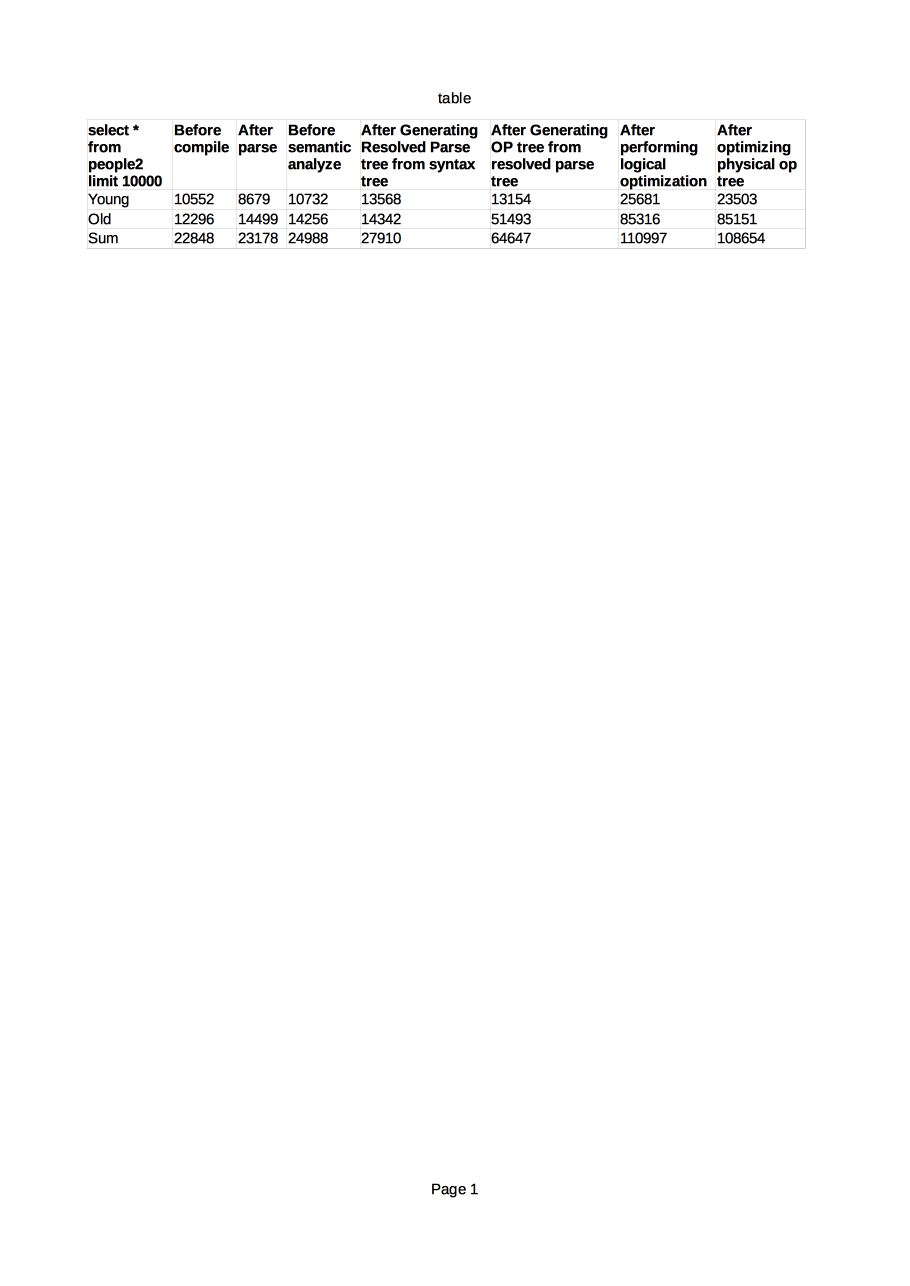
\includegraphics[width=150mm, keepaspectratio]{figures/parse_output.png}
	\centering
	\caption{Sample output of the parsing}
\end{figure}


\subsection{How HiveServer2 uses memory}
I have the code to measure the memory of Hive and get anget a general picture of the usage at certain phases. With this I am able to get a better understanding when and why memory goes high. I would like to get an answer to these querstions: How does the number of joins increase the memory? Which type of query generates a lot of memory usage: union, group by? If we increase the number of partitions, how it effects the heap size? In this section these questions will be answered.

The first step is to create a managed table where I will run my queries in the future. Hive faces memory problems when we have a highly partitioned table. I decided that for the first run, 20 000 partitions will be enough. 

